\documentclass[12pt]{amsart}
      % \newif\ifpreview
      % \previewfalse

% approx iid
\newcommand\simiid{\stackrel{\mathclap{\normalfont\mbox{\tiny{iid}}}}{\sim}}
\usepackage{natbib}
\usepackage{titlecaps}
\Addlcwords{a about above after again against all am an and any are aren't as at be because been before being below between both but by can't cannot could couldn't did didn't do does doesn't doing don't down during each few for from further had hadn't has hasn't have haven't having he he'd he'll he's her here here's hers herself him himself his how how's i i'd i'll i'm i've if in into is isn't it it's its itself let's me more most mustn't my myself no nor not of off on once only or other ought our ours ourselves out over own same shan't she she'd she'll she's should shouldn't so some such than that that's the their theirs them themselves then there there's these they they'd they'll they're they've this those through to too under until up very was wasn't we we'd we'll we're we've were weren't what what's when when's where where's which while who who's whom why why's with won't would wouldn't you you'd you'll you're you've your yours yourself yourselves}

% Fonts
% at some point figure out bolding ...
\usepackage[default,oldstyle,scale=0.95]{opensans}
%\usepackage[sfdefault,scaled=.85]{FiraSans}
\usepackage[T1]{fontenc}
\usepackage{textcomp}
\usepackage[varqu,varl]{zi4}% inconsolata typewriter
\usepackage{amsmath,amsthm}
\usepackage[cmintegrals]{newtxsf}
\usepackage[T1]{fontenc}
\usepackage{ae}

% easy commands for number propers
\newcommand{\first}{1$^{\text{st}}$}
\newcommand{\second}{2$^{\text{nd}}$}
\newcommand{\third}{3$^{\text{rd}}$}
\newcommand{\nth}[1]{${#1}^{\text{th}}$}

% Generate some fake text
\usepackage{blindtext}

% % add watermark
% \usepackage{draftwatermark}
% \SetWatermarkText{Submission Copy}
% \SetWatermarkScale{.5}
% \SetWatermarkColor[gray]{0.9}

% layout control
\usepackage{geometry}
\geometry{verbose,tmargin=1in,bmargin=1.25in,lmargin=1in,rmargin=1in}
\usepackage{parallel}
\usepackage{parcolumns}
\usepackage{fancyhdr}
\usepackage[export]{adjustbox}
\usepackage{etoolbox}

% math typesetting
\usepackage{array}
\usepackage{amsmath}
\usepackage{amssymb}
\usepackage{amsthm}
\usepackage{amsfonts}
\usepackage{relsize}
\usepackage{mathtools}
\usepackage{bm}
%\usepackage[%decimalsymbol=.,digitsep=fullstop]{siunitx}

% restricts float objects to be inserted before end of section
% creates float barriers
\usepackage[section]{placeins}

% tables
\usepackage{tabularx}
\usepackage{booktabs}
\usepackage{multicol}
\usepackage{multirow}
\usepackage{longtable}

% to adapt caption style
\usepackage[font={small},labelfont=bf]{caption}

% footnotes at bottom
%\usepackage[bottom]{footmisc}

% to change enumeration symbols begin{enumerate}[(a)]
\usepackage{enumerate}
\usepackage{paralist}

% to colorize links in document. See color specification below
\usepackage[pdftex,hyperref,x11names]{xcolor}

% for multiple references and insertion of the word "figure" or "table"
% \usepackage{cleveref}

% load the hyper-references package and set document info
\usepackage[pdftex]{hyperref}

% graphics stuff
\usepackage{subfigure}
\usepackage{graphicx}
\usepackage[space]{grffile} % allows us to specify directories that have spaces
\usepackage{placeins} % prevents floats from moving past a \FloatBarrier
\usepackage{tikz}

% sideway figures
\usepackage{rotating}
\usepackage{lscape}

%\usepackage[figuresright]{rotating}
% \newenvironment{amssidewaysfigure}  {\begin{sidewaysfigure}\vspace*{.8\textwidth}\begin{minipage}{\textheight}\centering}
%   {\end{minipage}\end{sidewaysfigure}}

% Spacing
\usepackage[doublespacing]{setspace}

% outside code
\usepackage{listings}
\usepackage{enumitem}

% define clickable links and their colors
\hypersetup{%
	unicode=false,          % non-Latin characters in Acrobat's bookmarks
	pdftoolbar=true,        % show Acrobat's toolbar?
	pdfmenubar=true,        % show Acrobat's menu?
	pdffitwindow=false,     % window fit to page when opened
	pdfstartview={FitH},    % fits the width of the page to the window
	pdfnewwindow=true,%
	%pagebackref=false,%
	pdfauthor={Shahryar Minhas, et alia.},%
	pdftitle={Taking Dyads Seriously},%
	colorlinks,%
	citecolor=black,%
	filecolor=black,%
	linkcolor=black,%
	urlcolor=RoyalBlue4
}

% -------------------- title -------------------- %

\title{Taking Dyads Seriously}
\vspace{\baselineskip}

% \author[Minhas]{Shahryar Minhas}
% \address{Shahryar Minhas: Department of Political Science}
% \curraddr{Michigan State University}
% \email[Corresponding author]{minhassh@msu.edu}

% \author[Dorff]{Cassy L. Dorff}
% \address{Cassy L. Dorff}
% \curraddr{Department of Political Science, University of New Mexico}
% \email{cdorff@unm.edu}

% \author[Foster]{Margaret Foster}
% \address{Margaret Foster}
% \curraddr{Department of Political Science, Duke University}
% \email{margaret.foster@duke.edu}

% \author[Gallop]{Max Gallop}
% \address{Max Gallop}
% \curraddr{Department of Government and Public Policy, University of Strathclyde}
% \email{max.gallop@strath.ac.uk}

% \author[Liu]{Howard Liu}
% \address{Howard Liu}
% \curraddr{Department of Political Science, Duke University}
% \email{hao.liu@duke.edu}

% \author[Tellez]{Juan Tellez}
% \address{Juan Tellez}
% \curraddr{Department of Political Science, Duke University}
% \email{juan.tellez@duke.edu}

% \author[Ward]{Michael D. Ward}
% \address{Michael D. Ward}
% \curraddr{Department of Political Science, Duke University}
% \email{michael.d.ward@duke.edu}

% \date{\today}

% \thanks{Shahryar Minhas and Michael D. Ward acknowledge support from National Science Foundation (NSF) Award 1259266. Peter Hoff, John Ahlquist, Robert Franzese, Arturas Rozenas, Betsy Sinclair, Jacob Montgomery and Benjamin Appel provided welcome and helpful comments. We also thank Douglas Gibler for kindly providing us with a copy of the data and programs he used in \citet{gibler:2017}. We benefited from presentations of this material at the 2017 Political Methodology Conference, and our home institutions.}

\setlength{\headheight}{15pt}
\setlength{\headsep}{20pt}
\pagestyle{fancyplain}
\fancyhf{}
\lhead{\fancyplain{}{}}
% \chead{\fancyplain{}{Taking Dyads Seriously}}
\chead{\fancyplain{}{}}
% \rhead{\fancyplain{}{\today}}
\rhead{\fancyplain{}{}}
\rfoot{\fancyplain{}{\thepage}}

% references to graphics
\makeatletter
% \def\input@path{{/Users/janus829/Dropbox/toDo_notes/nsfSumm/Graphics/}, {/Users/s7m/Dropbox/toDo_notes/nsfSumm/Graphics/}}
% \graphicspath{{/Users/janus829/Dropbox/toDo_notes/nsfSumm/Graphics/}, {/Users/s7m/Dropbox/toDo_notes/nsfSumm/Graphics/}}

% easy command for boldface math symbols
\newcommand{\mbs}[1]{\boldsymbol{#1}}

% command for R package font
\newcommand{\pkg}[1]{{\fontseries{b}\selectfont #1}}

% Add some colors
\definecolor{red1}{RGB}{253,219,199}
\definecolor{red2}{RGB}{244,165,130}
\definecolor{red3}{RGB}{178,24,43}

\definecolor{green1}{RGB}{229,245,224}
\definecolor{green2}{RGB}{161,217,155}
\definecolor{green3}{RGB}{49,163,84}

\definecolor{blue0}{RGB}{255,247,251}
\definecolor{blue1}{RGB}{222,235,247}
\definecolor{blue2}{RGB}{158,202,225}
\definecolor{blue3}{RGB}{49,130,189}
\definecolor{blue4}{RGB}{4,90,141}

\definecolor{purple1}{RGB}{191,211,230}
\definecolor{purple2}{RGB}{140,150,198}
\definecolor{purple3}{RGB}{140,107,177}

\definecolor{brown1}{RGB}{246,232,195}
\definecolor{brown2}{RGB}{223,194,125}
\definecolor{brown3}{RGB}{191,129,45}

% square bracket matrices
\let\bbordermatrix\bordermatrix
\patchcmd{\bbordermatrix}{8.75}{4.75}{}{}
\patchcmd{\bbordermatrix}{\left(}{\left[}{}{}
\patchcmd{\bbordermatrix}{\right)}{\right]}{}{}


\begin{document}
% \ifpreview {
%    \definecolor{personal}{rgb}{1.0, 1.0, 0.0}
%    \pagecolor{personal}
%    }
% \fi


\small{\singlespacing{
\begin{abstract}
	International relations scholarship concerns dyads, yet standard modeling approaches fail to adequately capture the data generating process behind dyadic events and processes. As a result, they suffer from biased coefficients and poorly calibrated standard errors. We show how a regression-based approach, the Additive and Multiplicative Effects (AME) model, can be used to account for the inherent dependencies in dyadic data and glean substantive insights in the interrelations between actors. First, we conduct a simulation to highlight how the model captures dependencies and show that accounting for these processes improves our ability to conduct inference on dyadic data. Second, we compare the AME model to approaches used in three prominent studies from recent international relations scholarship. For each study, we find that compared to AME, the modeling approach used performs notably worse at capturing the data generating process. Further, conventional methods misstate the effect of key variables and the uncertainty in these effects. Finally, AME outperforms standard approaches in terms of out-of-sample fit. In sum, our work shows the consequences of failing to take the dependencies inherent to dyadic data seriously. Most importantly, by better modeling the data generating process underlying political phenomena, the AME framework improves scholars' ability to conduct inferential analyses on dyadic data.
\end{abstract}
}}


\maketitle

\begin{center}
	\textbf{Word count}: 9,542
\end{center}

\thispagestyle{empty}
\newpage\setcounter{page}{1}

\appendix
\clearpage

\renewcommand{\thefigure}{A\arabic{figure}}
\setcounter{figure}{0}
\renewcommand{\thetable}{A.\arabic{table}}
\setcounter{table}{0}
\renewcommand{\thesection}{A.\arabic{section}}
\setcounter{section}{0}

\section*{\textbf{Appendix}}

\subsection*{Additional Replication Information}

\subsubsection*{Gibler (2017)}

Coefficient plot and performance comparison.

% latex table generated in R 3.4.1 by xtable 1.8-2 package
% Sat Oct 21 23:10:24 2017
\begin{table}[ht]
\centering
\begingroup\normalsize
\begin{tabular}{lccc}
 Variable & GLM (Logit) & GLM (Probit) & AME \\ 
  \hline
\hline
(Intercept) & $-5.826$ & $-2.793$ & $-2.758$ \\
   & (0.366) & (0.366) & (0.045) \\ 
  Allied & 0.133 & 0.067 & $0.078$ \\
   & (0.102) & (0.102) & (0.021) \\ 
  Joint Democracy & $-0.527$ & $-0.186$ & 0.005 \\
   & (0.099) & (0.099) & (0.022) \\ 
  Peace Years & $-0.261$ & $-0.099$ & $-0.058$ \\
   & (0.016) & (0.016) & (0.004) \\ 
  Spline 1 & $-0.001$ & $0.000$ & $0.000$ \\
   & (0.000) & (0.000) & (0.000) \\ 
  Spline 2 & $0.000$ & $0.000$ & $0.000$ \\
   & (0.000) & (0.000) & (0.000) \\ 
  Spline 3 & 0.000 & 0.000 & $0.000$ \\
   & (0.000) & (0.000) & (0.000) \\ 
  Contiguity & $2.427$ & $0.95$ & $0.66$ \\
   & (0.196) & (0.196) & (0.023) \\ 
  Parity & -0.77 & -0.228 & -0.067 \\ 
   & (0.551) & (0.551) & (0.057) \\ 
  Parity at Entry Year & $2.034$ & 0.739 & -0.05 \\
   & (0.617) & (0.617) & (0.065) \\ 
  Rivalry & $2.034$ & $1.035$ & $0.655$ \\
   & (0.213) & (0.213) & (0.028) \\ 
   \hline
\hline
\end{tabular}
\endgroup
\caption{Parameter comparison for Gibler (2017). Standard errors in parentheses.} 
\label{tab:gibler_coef}
\end{table}

\FloatBarrier

\begin{figure}
	\centering   
	\subfigure[AUC]{\label{fig:giblerroc}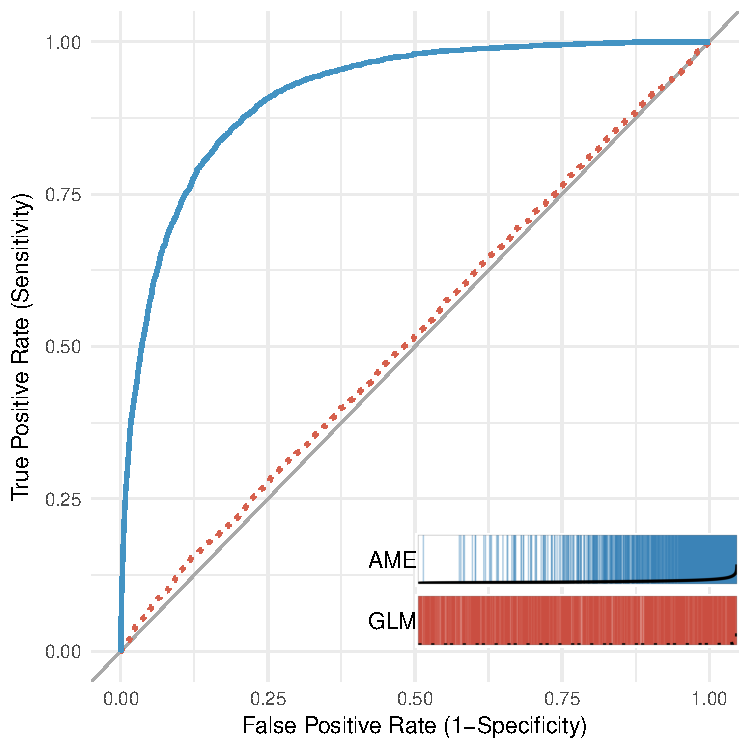
\includegraphics[width=.45\textwidth]{gibler_roc_outSample.pdf}}
	\subfigure[Precision and Recall]{\label{fig:giblerpr}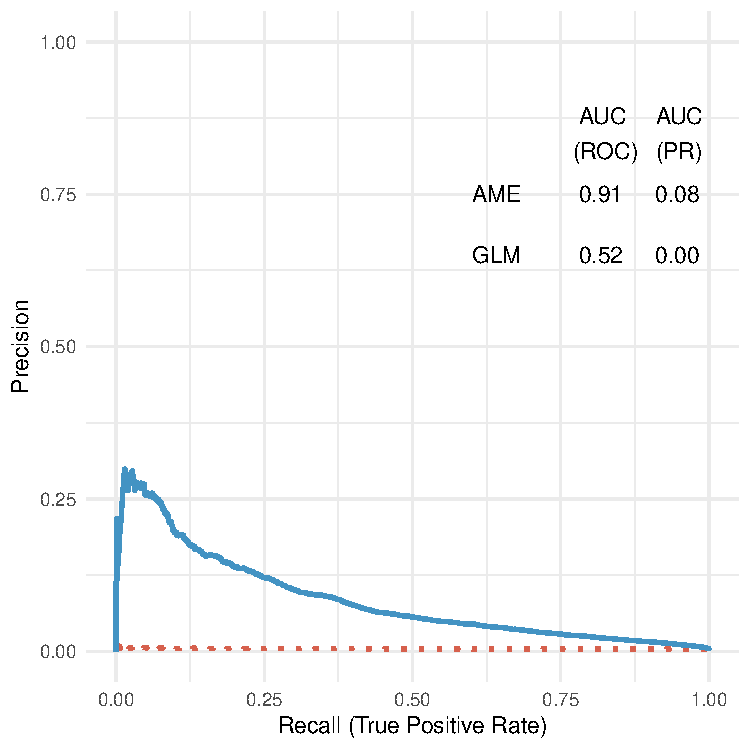
\includegraphics[width=.45\textwidth]{gibler_pr_outSample.pdf}}
	\caption{Assessments of out-of-sample predictive performance for Gibler (2017) using ROC curves and PR curves.}
\end{figure}
\FloatBarrier

\clearpage
\subsubsection*{McDonald (2004)}

Coefficient plot and performance comparison.

% latex table generated in R 3.4.1 by xtable 1.8-2 package
% Sat Oct 21 23:10:32 2017
\begin{table}[ht]
\centering
\begingroup\normalsize
\begin{tabular}{lccc}
 Variable & GLM (Logit) & GLM (Probit) & AME \\ 
  \hline
\hline
(Intercept) & 0.054 & 0.085 & $-1.171^{\ast\ast}$ \\ 
   & (1.179) & (0.409) & (0.096) \\ 
  Spline0 & $-0.438^{\ast\ast}$ & $-0.222^{\ast\ast}$ & $-0.145^{\ast\ast}$ \\ 
   & (0.061) & (0.026) & (0.019) \\ 
  Spline1 & $-0.003^{\ast\ast}$ & $-0.002^{\ast\ast}$ & $-0.001^{\ast\ast}$ \\ 
   & (0.001) & (0.000) & (0.000) \\ 
  Spline2 & 0.001 & $0.001^{\ast\ast}$ & $0.000^{\ast}$ \\ 
   & (0.001) & (0.000) & (0.000) \\ 
  Spline3 & 0.000 & 0.000 & $0.000^{\ast\ast}$ \\ 
   & (0.000) & (0.000) & (0.000) \\ 
  Shared Alliance & $0.483^{\ast\ast}$ & 0.155 & $0.342^{\ast\ast}$ \\ 
   & (0.233) & (0.095) & (0.069) \\ 
  Contiguous & $2.011^{\ast\ast}$ & $0.789^{\ast\ast}$ & $0.988^{\ast\ast}$ \\ 
   & (0.343) & (0.118) & (0.066) \\ 
  Log Capabilities Ratio & $-0.146^{\ast\ast}$ & $-0.054^{\ast\ast}$ & $0.029^{\ast\ast}$ \\ 
   & (0.072) & (0.026) & (0.013) \\ 
  Trade Dependence & -22.244 & -7.051 & $-13.134^{\ast\ast}$ \\ 
   & (15.184) & (5.536) & (4.938) \\ 
  Preconflict GDP Change & $-6.79^{\ast\ast}$ & $-3.155^{\ast\ast}$ & $-2.651^{\ast\ast}$ \\ 
   & (2.033) & (0.788) & (0.574) \\ 
  Lowest Dyadic Polity Score & $-0.036^{\ast\ast}$ & $-0.014^{\ast\ast}$ & $-0.026^{\ast\ast}$ \\ 
   & (0.015) & (0.006) & (0.002) \\ 
  Capabilities & $-0.995^{\ast\ast}$ & $-0.349^{\ast\ast}$ & 0.022 \\ 
   & (0.377) & (0.14) & (0.079) \\ 
  Logged GDP & $0.000^{\ast\ast}$ & $0.000^{\ast\ast}$ & $0.000^{\ast\ast}$ \\ 
   & (0.000) & (0.000) & (0.000) \\ 
  Logged Cap. Distance & $-0.425^{\ast\ast}$ & $-0.224^{\ast\ast}$ & $-0.275^{\ast\ast}$ \\ 
   & (0.14) & (0.047) & (0.012) \\ 
  Major Power In Dyad & $0.769^{\ast\ast}$ & $0.312^{\ast\ast}$ & $0.212^{\ast\ast}$ \\ 
   & (0.322) & (0.122) & (0.098) \\ 
  Higest Barrier To Trade & $0.024^{\ast\ast}$ & $0.011^{\ast\ast}$ & $0.004^{\ast\ast}$ \\ 
   & (0.008) & (0.003) & (0.001) \\ 
   \hline
\hline
\end{tabular}
\endgroup
\caption{Parameter comparison for McDonald (2004). Standard errors in parentheses. $^{**}$ and $^{*}$ indicate significance at $p<0.05$ and $p<0.10$, respectively.} 
\label{tab:mcdonald_coef}
\end{table}

\FloatBarrier

\begin{figure}
	\centering   
	\subfigure[AUC]{\label{fig:mcdonaldroc}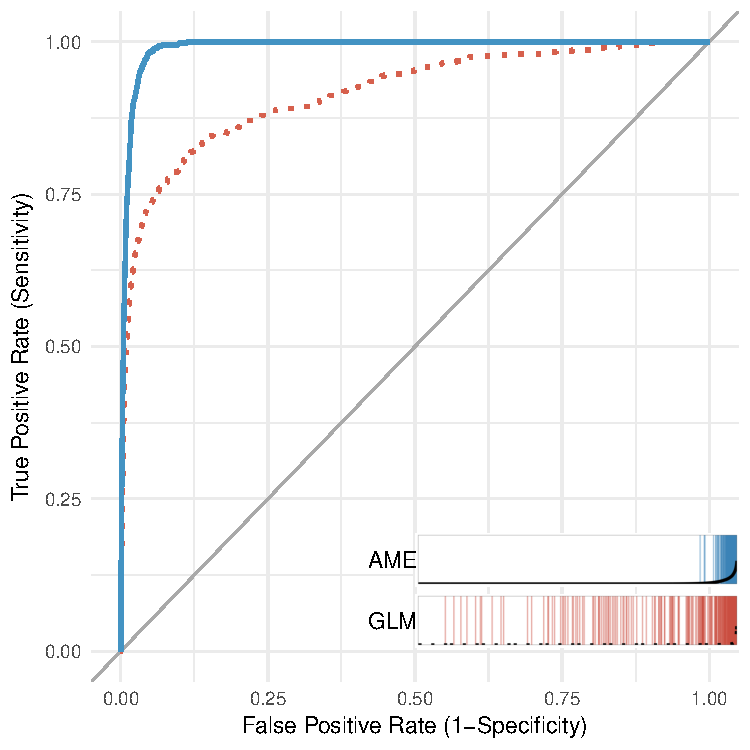
\includegraphics[width=.45\textwidth]{mcdonald_roc_outSample.pdf}}
	\subfigure[Precision and Recall]{\label{fig:mcdonaldpr}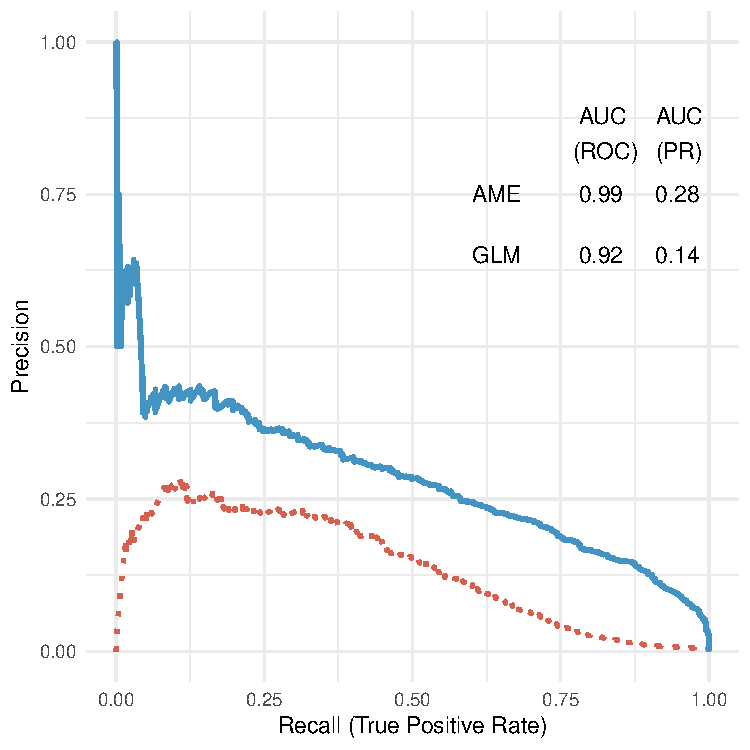
\includegraphics[width=.45\textwidth]{mcdonald_pr_outSample.pdf}}
	\caption{Assessments of out-of-sample predictive performance for McDonald (2004) using ROC curves and PR curves.}
\end{figure}
\FloatBarrier

\clearpage
\subsubsection*{Reiter \& Stam (2003)}

Coefficient plot and performance comparison.

% latex table generated in R 3.4.1 by xtable 1.8-2 package
% Sat Oct 21 23:16:42 2017
\begin{table}[ht]
\centering
\begingroup\normalsize
\begin{tabular}{lccc}
 Variable & GLM (Logit) & GLM (Probit) & AME \\ 
  \hline
\hline
Intercept & $-4.784^{\ast\ast}$ & $-2.339^{\ast\ast}$ & $-3.144^{\ast\ast}$ \\ 
   & (0.097) & (0.034) & (0.06) \\ 
  Pers/Democ Directed Dyad & $1.026^{\ast\ast}$ & $0.378^{\ast\ast}$ & $0.255^{\ast\ast}$ \\ 
   & (0.14) & (0.051) & (0.068) \\ 
  Democ/Pers Directed Dyad & 0.083 & 0.033 & 0.112 \\ 
   & (0.191) & (0.066) & (0.079) \\ 
  Personal & 0.281 & 0.15 & $0.211^{\ast}$ \\ 
   & (0.265) & (0.099) & (0.11) \\ 
  Military & -0.323 & -0.105 & -0.025 \\ 
   & (0.574) & (0.204) & (0.249) \\ 
  Single & $-0.677^{\ast\ast}$ & $-0.261^{\ast\ast}$ & -0.07 \\ 
   & (0.144) & (0.062) & (0.073) \\ 
  Democracy & $-1.073^{\ast\ast}$ & $-0.428^{\ast\ast}$ & $-0.254^{\ast\ast}$ \\ 
   & (0.194) & (0.07) & (0.063) \\ 
  Contiguous & $2.912^{\ast\ast}$ & $1.147^{\ast\ast}$ & $1.296^{\ast\ast}$ \\ 
   & (0.09) & (0.031) & (0.033) \\ 
  Major Power & $2.174^{\ast\ast}$ & $0.919^{\ast\ast}$ & $0.906^{\ast\ast}$ \\ 
   & (0.101) & (0.037) & (0.093) \\ 
  Ally & 0.078 & -0.003 & $0.136^{\ast\ast}$ \\ 
   & (0.086) & (0.035) & (0.037) \\ 
  Higher/Lower Power Ratio & $-0.316^{\ast\ast}$ & $-0.122^{\ast\ast}$ & $-0.111^{\ast\ast}$ \\ 
   & (0.027) & (0.01) & (0.011) \\ 
  Economically Advanced & -0.175 & -0.054 & 0.053 \\ 
   & (0.131) & (0.051) & (0.05) \\ 
  Years Since Last Dispute & $-0.381^{\ast\ast}$ & $-0.149^{\ast\ast}$ & $-0.129^{\ast\ast}$ \\ 
   & (0.023) & (0.009) & (0.008) \\ 
  Cubic Spline 1 & $-0.004^{\ast\ast}$ & $-0.001^{\ast\ast}$ & $-0.001^{\ast\ast}$ \\ 
   & (0.000) & (0.000) & (0.000) \\ 
  Cubic Spline 2 & $0.002^{\ast\ast}$ & $0.001^{\ast\ast}$ & $0.001^{\ast\ast}$ \\ 
   & (0.000) & (0.000) & (0.000) \\ 
  Cubic Spline 3 & $-0.001^{\ast\ast}$ & $0.000^{\ast\ast}$ & $0.000^{\ast\ast}$ \\ 
   & (0.000) & (0.000) & (0.000) \\ 
   \hline
\hline
\end{tabular}
\endgroup
\caption{Parameter comparison for Reiter \& Stam (2003). Standard errors in parentheses. $^{**}$ and $^{*}$ indicate significance at $p<0.05$ and $p<0.10$, respectively.} 
\label{tab:reiter_stam_coef}
\end{table}
\FloatBarrier

\begin{figure}
	\centering   
	\subfigure[AUC]{\label{fig:reiterstamroc}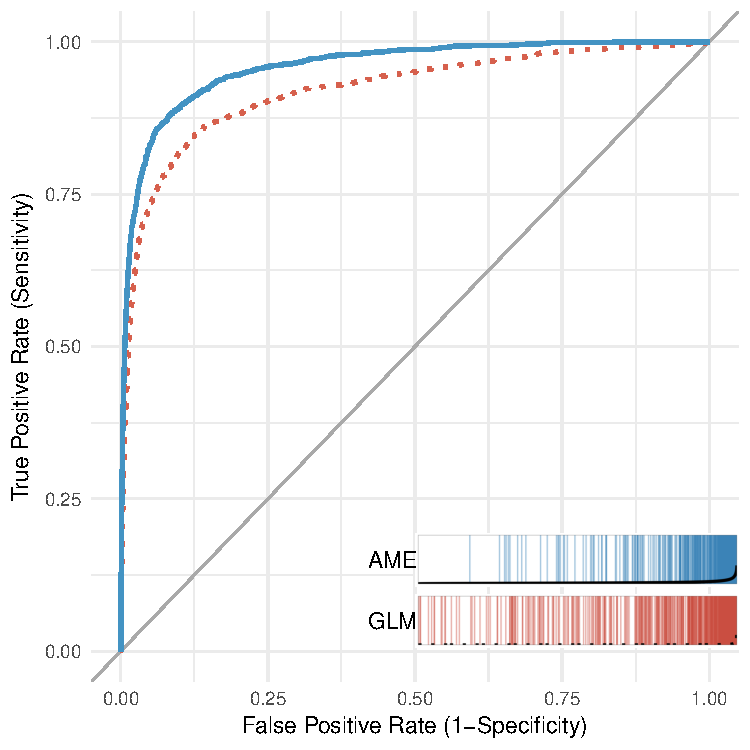
\includegraphics[width=.45\textwidth]{reiter_stam_roc_outSample.pdf}}
	\subfigure[Precision and Recall]{\label{fig:reiterstampr}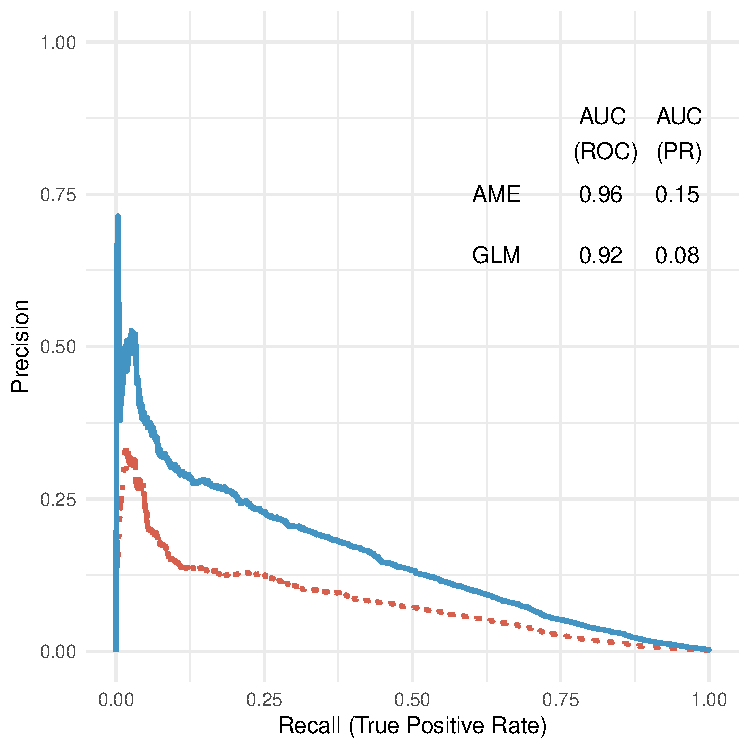
\includegraphics[width=.45\textwidth]{reiter_stam_pr_outSample.pdf}}
	\caption{Assessments of out-of-sample predictive performance for Reiter \& Stam (2003) using ROC curves and PR curves.}
\end{figure}
\FloatBarrier

\clearpage
\subsubsection*{Rose (2004)}

Coefficient plot and performance comparison.

% latex table generated in R 3.4.1 by xtable 1.8-2 package
% Sat Oct 21 22:58:31 2017
\begin{table}[ht]
\centering
\begingroup\normalsize
\begin{tabular}{lcc}
 Variable & LM & AME \\ 
  \hline
\hline
Intercept & $-24.96^{\ast\ast}$ & $-22.532^{\ast\ast}$ \\ 
   & (0.409) & (0.103) \\ 
  Both in GATT/WTO & -0.042 & $-0.56^{\ast\ast}$ \\ 
   & (0.053) & (0.013) \\ 
  One in GATT/WTO & -0.058 & $-0.317^{\ast\ast}$ \\ 
   & (0.049) & (0.012) \\ 
  GSP & $0.859^{\ast\ast}$ & $0.399^{\ast\ast}$ \\ 
   & (0.032) & (0.009) \\ 
  Log Distance & $-1.119^{\ast\ast}$ & $-1.097^{\ast\ast}$ \\ 
   & (0.022) & (0.005) \\ 
  Log Product Real GDP & $0.916^{\ast\ast}$ & $0.798^{\ast\ast}$ \\ 
   & (0.01) & (0.002) \\ 
  Log Product Real GDPpc & $0.321^{\ast\ast}$ & $0.244^{\ast\ast}$ \\ 
   & (0.014) & (0.004) \\ 
  Regional FTA & $1.199^{\ast\ast}$ & $0.826^{\ast\ast}$ \\ 
   & (0.106) & (0.027) \\ 
  Currency Union & $1.118^{\ast\ast}$ & $1.144^{\ast\ast}$ \\ 
   & (0.122) & (0.029) \\ 
  Common language & $0.313^{\ast\ast}$ & $0.345^{\ast\ast}$ \\ 
   & (0.04) & (0.009) \\ 
  Land Border & $0.526^{\ast\ast}$ & $0.483^{\ast\ast}$ \\ 
   & (0.111) & (0.02) \\ 
  Number Landlocked & $-0.271^{\ast\ast}$ & $-0.42^{\ast\ast}$ \\ 
   & (0.031) & (0.009) \\ 
  Number Islands & 0.042 & $0.058^{\ast\ast}$ \\ 
   & (0.036) & (0.009) \\ 
  Log Product Land Area & $-0.097^{\ast\ast}$ & $-0.024^{\ast\ast}$ \\ 
   & (0.008) & (0.002) \\ 
  Common Colonizer & $0.585^{\ast\ast}$ & $0.418^{\ast\ast}$ \\ 
   & (0.067) & (0.013) \\ 
  Currently Colonized & $1.075^{\ast\ast}$ & $1.762^{\ast\ast}$ \\ 
   & (0.235) & (0.081) \\ 
  Ever Colony & $1.164^{\ast\ast}$ & $1.335^{\ast\ast}$ \\ 
   & (0.117) & (0.024) \\ 
  Common Country & -0.016 & $-0.672^{\ast\ast}$ \\ 
   & (1.097) & (0.19) \\ 
   \hline
\hline
\end{tabular}
\endgroup
\caption{Parameter comparison for Rose (2004). Standard errors in parentheses. $^{**}$ and $^{*}$ indicate significance at $p<0.05$ and $p<0.10$, respectively.} 
\label{tab:rose_coef}
\end{table}

\FloatBarrier

% \begin{figure}
% 	\centering   
% 	\subfigure[AUC]{\label{fig:reitaucpr}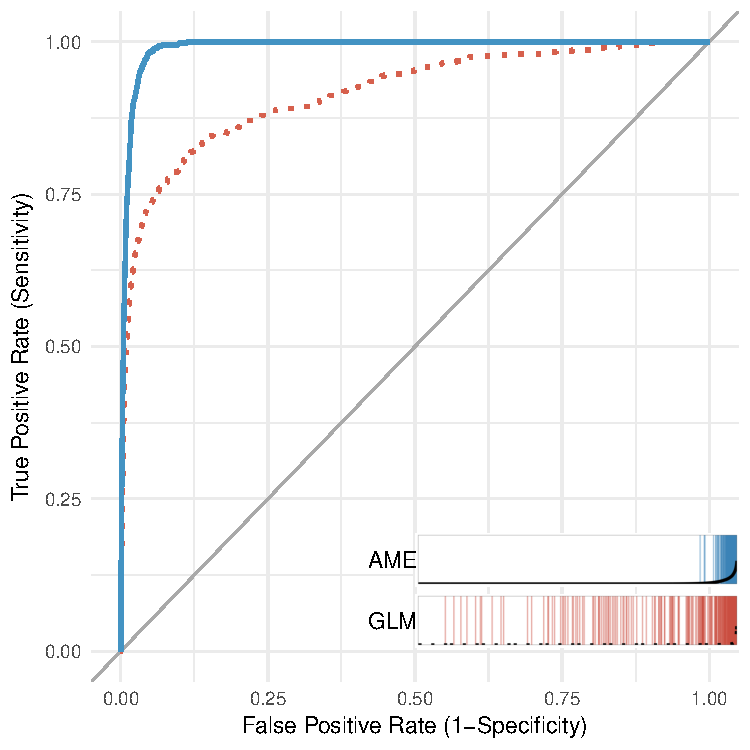
\includegraphics[width=.45\textwidth]{mcdonald_roc_outSample.pdf}}
% 	\subfigure[Precision and Recall]{\label{fig:reitpr}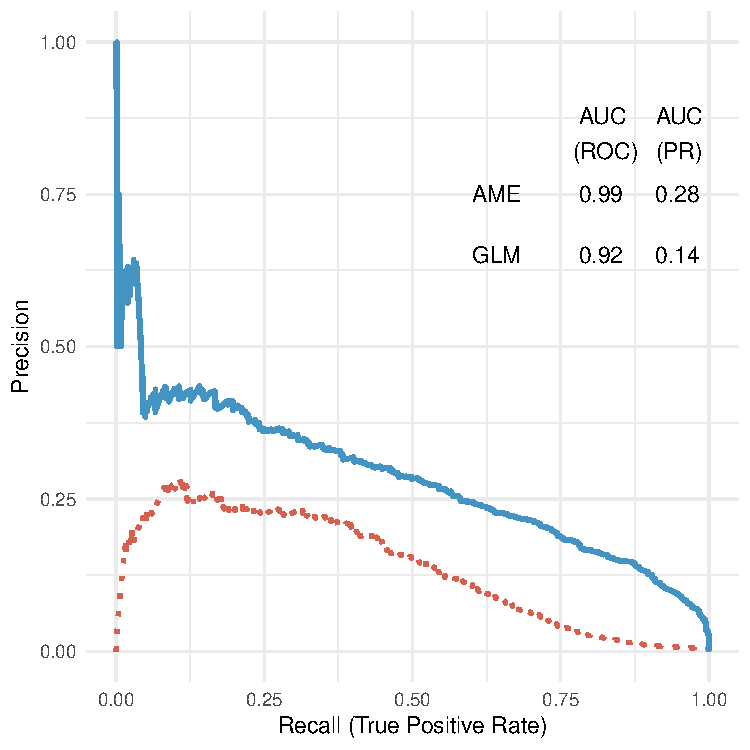
\includegraphics[width=.45\textwidth]{mcdonald_pr_outSample.pdf}}
% 	\caption{Assessments of out-of-sample predictive performance for McDonald (2004) using ROC curves and PR curves.}
% \end{figure}
\FloatBarrier

\clearpage
\subsubsection*{Weeks (2012)}

Coefficient plot and performance comparison.

% latex table generated in R 3.4.1 by xtable 1.8-2 package
% Sat Oct 21 23:26:08 2017
\begin{table}[ht]
\centering
\begingroup\scriptsize
\begin{tabular}{lccc}
 Variable & GLM (Logit) & GLM (Probit) & AME \\ 
  \hline
\hline
(Intercept) & $-3.784^{\ast\ast}$ & $-1.797^{\ast\ast}$ & $-2.409^{\ast\ast}$ \\ 
   & (0.423) & (0.159) & (0.132) \\ 
  Machine & $-0.459^{\ast\ast}$ & $-0.162^{\ast\ast}$ & -0.006 \\ 
   & (0.174) & (0.062) & (0.04) \\ 
  Junta & $0.515^{\ast\ast}$ & $0.194^{\ast\ast}$ & 0.034 \\ 
   & (0.169) & (0.062) & (0.046) \\ 
  Boss & $0.649^{\ast\ast}$ & $0.281^{\ast\ast}$ & -0.044 \\ 
   & (0.153) & (0.05) & (0.044) \\ 
  Strongman & $0.832^{\ast\ast}$ & $0.295^{\ast\ast}$ & 0.032 \\ 
   & (0.132) & (0.048) & (0.044) \\ 
  Other Type & 0.147 & 0.051 & -0.01 \\ 
   & (0.132) & (0.046) & (0.034) \\ 
  New/Unstable Regime & $-0.312^{\ast\ast}$ & $-0.123^{\ast\ast}$ & -0.043 \\ 
   & (0.092) & (0.033) & (0.031) \\ 
  Democracy Target & 0.185 & 0.052 & 0.024 \\ 
   & (0.115) & (0.04) & (0.026) \\ 
  Military Capabilities Initiator & $5.234^{\ast\ast}$ & $2.136^{\ast\ast}$ & 0.071 \\ 
   & (1.69) & (0.554) & (0.412) \\ 
  Military Capabilities Target  & $6.34^{\ast\ast}$ & $2.865^{\ast\ast}$ & $-0.969^{\ast\ast}$ \\ 
   & (1.675) & (0.573) & (0.48) \\ 
  Low Trade Dependence  & $-24.794^{\ast}$ & -8.197 & -4.733 \\ 
   & (12.866) & (5.582) & (3.017) \\ 
  Both Major Powers & $1.136^{\ast\ast}$ & $0.687^{\ast\ast}$ & $1.122^{\ast\ast}$ \\ 
   & (0.547) & (0.183) & (0.241) \\ 
  Minor/Major & $0.772^{\ast\ast}$ & $0.292^{\ast\ast}$ & $0.496^{\ast\ast}$ \\ 
   & (0.239) & (0.086) & (0.118) \\ 
  Major/Minor & $0.711^{\ast\ast}$ & $0.332^{\ast\ast}$ & $0.778^{\ast\ast}$ \\ 
   & (0.225) & (0.075) & (0.16) \\ 
  Contiguous & $2.172^{\ast\ast}$ & $0.738^{\ast\ast}$ & $0.705^{\ast\ast}$ \\ 
   & (0.32) & (0.125) & (0.06) \\ 
  Log Dist. Between Capitals & $-0.209^{\ast\ast}$ & $-0.095^{\ast\ast}$ & $-0.129^{\ast\ast}$ \\ 
   & (0.038) & (0.015) & (0.01) \\ 
  Alliance Similarity Dyad  & $-0.999^{\ast\ast}$ & $-0.386^{\ast\ast}$ & -0.073 \\ 
   & (0.144) & (0.05) & (0.065) \\ 
  Alliance Similarity With System Leader Initiator & 0.11 & 0.011 & 0.068 \\ 
   & (0.24) & (0.082) & (0.057) \\ 
  Alliance Similarity Leader Target & 0.203 & 0.032 & 0.08 \\ 
   & (0.244) & (0.081) & (0.056) \\ 
  Time Since Last Conflict & $-0.229^{\ast\ast}$ & $-0.089^{\ast\ast}$ & $-0.067^{\ast\ast}$ \\ 
   & (0.018) & (0.007) & (0.007) \\ 
  Spline1 & $-0.001^{\ast\ast}$ & $0.000^{\ast\ast}$ & $0.000^{\ast\ast}$ \\ 
   & (0.000) & (0.000) & (0.000) \\ 
  Spline2 & $0.000^{\ast\ast}$ & $0.000^{\ast\ast}$ & $0.000^{\ast\ast}$ \\ 
   & (0.000) & (0.000) & (0.000) \\ 
  Spline3 & 0.000 & 0.000 & 0.000 \\ 
   & (0.000) & (0.000) & (0.000) \\ 
   \hline
\hline
\end{tabular}
\endgroup
\caption{Parameter comparison for Weeks (2012). Standard errors in parentheses. $^{**}$ and $^{*}$ indicate significance at $p<0.05$ and $p<0.10$, respectively.} 
\label{tab:weeks_coef}
\end{table}

\FloatBarrier

% already show roc-pr in main text
% \begin{figure}
% 	\centering   
% 	\subfigure[AUC]{\label{fig:weeksroc}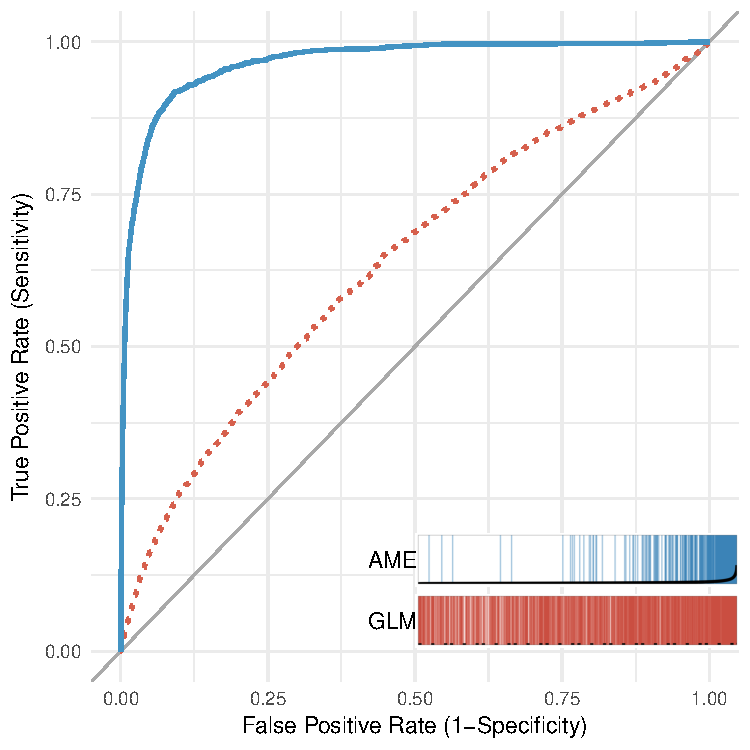
\includegraphics[width=.45\textwidth]{weeks_roc_outSample.pdf}}
% 	\subfigure[Precision and Recall]{\label{fig:weekspr}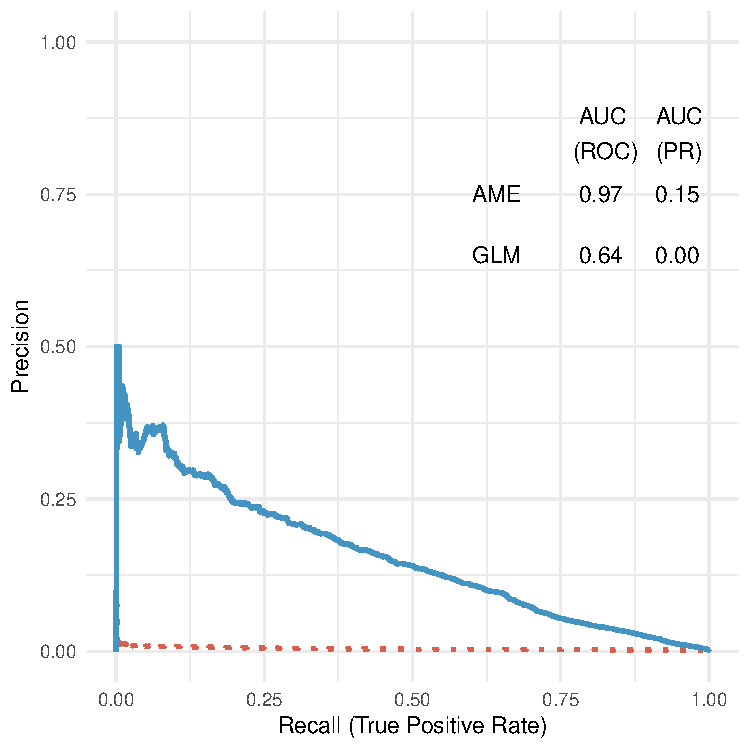
\includegraphics[width=.45\textwidth]{weeks_pr_outSample.pdf}}
% 	\caption{Assessments of out-of-sample predictive performance for Weeks (2012) using ROC curves and PR curves.}
% \end{figure}
% \FloatBarrier

\newpage
% Bib stuff
\clearpage

\bibliography{C:/Users/Owner/whistle/master}
% \bibliography{C:/Users/S7M/whistle/master}
% \bibliography{C:/Users/herme/whistle/master}
%\bibliography{/Users/s7m/whistle/master}
\bibliographystyle{authordate1}
% \bibliographystyle{sm}
% \clearpage
% \section*{All About Us}

\end{document}
